
\documentclass[10pt]{beamer}
% \usepackage{subfiles}

\usepackage[danish]{babel}
\usepackage[utf8]{inputenc}
\usetheme[progressbar=frametitle]{metropolis}
\usepackage{appendixnumberbeamer}


\usepackage{booktabs}
\usepackage[scale=2]{ccicons}

% \usepackage{pgfplots}
% \usepgfplotslibrary{dateplot}

\definecolor{Orange}{RGB}{229,134,25}

\usepackage{xspace}
\newcommand{\themename}{\textbf{\textsc{metropolis}}\xspace}
\usepackage{listings}


\definecolor{background}{RGB}{226, 226, 226}


\lstset{ 
literate=% 
{Ö}{{\"O}}1 
{Ä}{{\"A}}1 
{Ü}{{\"U}}1 
{ß}{{\ss}}{ 1\negmedspace\,} 
{ü}{{\"u}}1 
{ä}{{\"a}}1 
{ö}{{\"o}}1 
{ø}{{\o}}{1\negmedspace\,} 
{Ø}{{\O}}{1\negthinspace\,\,} 
{å}{{\aa}}{1\negthickspace\,} 
{Å}{{\AA}}{1\negthinspace\;} 
{æ}{{\ae}}{1\negthinspace\;} 
{Æ}{{\AE}}{1\,\,}}

\lstdefinestyle{terminal}{
	language=bash,
	aboveskip=2mm,
	belowskip=2mm,
	showstringspaces=false,
	columns=flexible,
	basicstyle={\small\ttfamily},
	numbers=none,
	numberstyle=\footnotesize,
	commentstyle=\color{black},
	frame=single,
	framesep=2pt,
	breaklines=true,
	breakatwhitespace=false,
	backgroundcolor = \color{background},
	tabsize=2
}


\lstdefinestyle{python}{
	language=Python,
	aboveskip=2mm,
	belowskip=1mm,
	showstringspaces=false,
	columns=flexible,
	numbers=none,
	numberstyle=\footnotesize,
	commentstyle=\ttfamily\color{black},
	frame=single,
	framesep=2pt,
	breaklines=true,
	breakatwhitespace=false,
	backgroundcolor = \color{background},
	tabsize=2
}



\title{Lær Python dag 1 - modul 1}
\subtitle{Introduktion, basis python}
% \date{\today}
\date{}
\author{Steffen Berg Klenow \\Jonas Bamse Andersen}
\institute{Syddansk Universitet}
% \titlegraphic{\hfill
\includegraphics[height=1.5cm]{logo.pdf}}


\title{Lær Python dag 2 - modul 1}
\subtitle{Løkker og lister}

\begin{document}

\maketitle

\begin{frame}{Indhold}
  \setbeamertemplate{section in toc}[sections numbered]
  \tableofcontents[hideallsubsections]
\end{frame}

\section{Recap}
\begin{frame}[fragile]{Certifikat}
Alle deltagere den sidste gang kan få et certifikat på deltagelse.
\begin{center}
	
\includegraphics[width=.8\textwidth]{certificate.pdf}
\end{center}
\end{frame}


\begin{frame}[fragile]{Hvad lærte I sidst?}
Diskutér to minutter med sidemanden, hvad I lærte sidst.

	\begin{itemize}
		\item Hvad er en type?
		\item Hvad er en variabel?
		\item Hvad er en if-sætning?
		\item Hvad er en funktion?
	\end{itemize}
\end{frame}

\begin{frame}[fragile]{Apropos funktioner}
	\begin{center}
		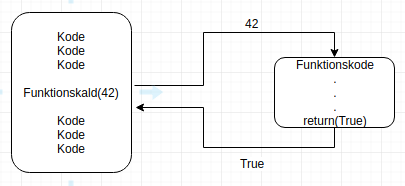
\includegraphics[width=0.8\textwidth]{figs/funcs.png}
	\end{center}
\pause
Lad os prøve at lave Fibonacci tallene.
\end{frame}

\section{Løkker}

\begin{frame}[fragile]{Tæl til 5}
	Hvordan kan vi skrive kode som tæller fra 1-5 (printer tallene)?
	\pause
	\begin{columns}
		\column{0.4\textwidth}
		\begin{lstlisting}[style=python]
print(1)
print(2)
print(3)
print(4)
print(5)
		\end{lstlisting}
		\column{0.4\textwidth}
		\begin{lstlisting}[style=python]
1
2
3
4
5
		\end{lstlisting}
	\end{columns}
	Virker umiddelbart lidt besværligt, hvad hvis det er en større mængde instruktioner vi vil have gentaget flere gange?\\
	Eller hvad med et variabelt antal gange?
\end{frame}

\begin{frame}[fragile]{Løkker}
	Vi kan gøre det med løkker!
	\begin{center}
		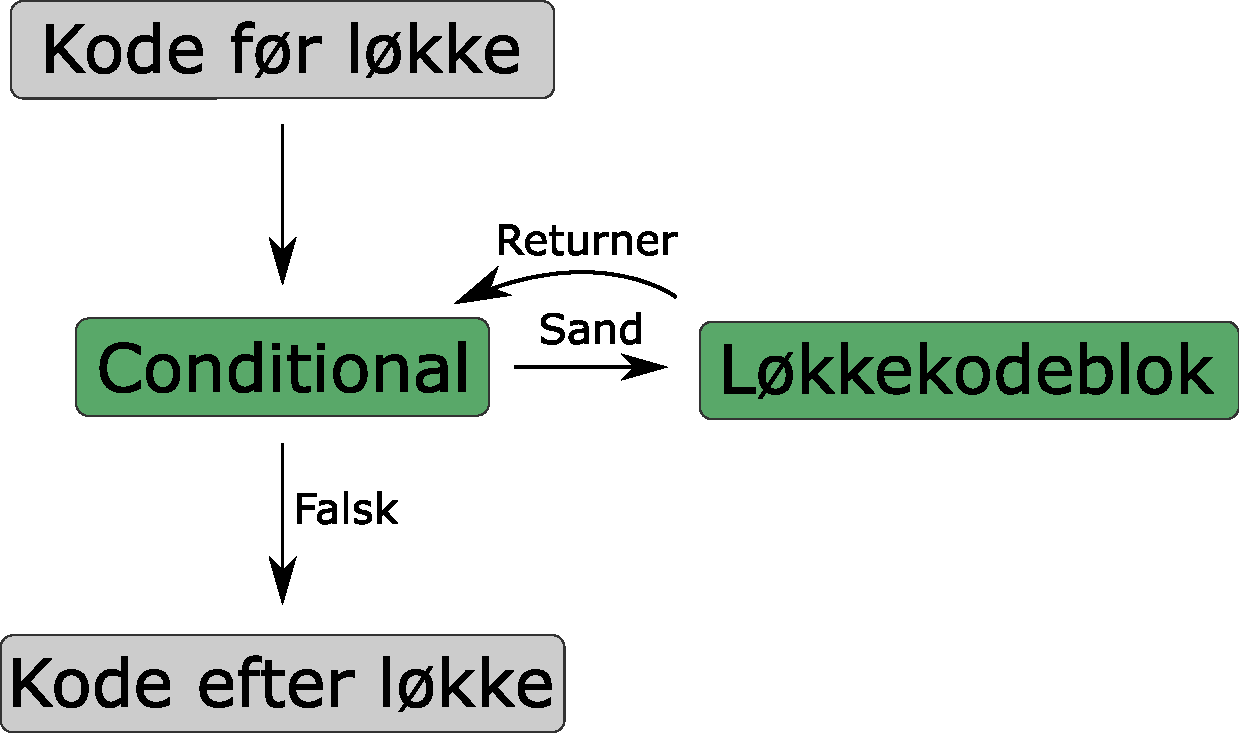
\includegraphics[width=0.8\textwidth]{figs/loop.pdf}
	\end{center}
\end{frame}


\begin{frame}[fragile]{For loop}
	Gentagelse et fast antal gange ved hjælp af for-løkke:
	\begin{lstlisting}[style=python]
for <variabel> in range(<antal>):
	<instruktion>
	<instruktion>
	<instruktion>
	\end{lstlisting}
	\pause
	Eksempel:
	\begin{columns}
		\column{0.4\textwidth}
		\begin{lstlisting}[style=python]
for i in range(5):
	print(i)
		\end{lstlisting}
		\column{0.4\textwidth}
		\begin{lstlisting}[style=python]
0
1
2
3
4
		\end{lstlisting}
	\end{columns}
\end{frame}


\begin{frame}[fragile]{For loop}
	Men hvad hvis vi gerne vil tælle fra 1 til 5?
	\pause
	\begin{columns}
		\column{0.4\textwidth}
		\begin{lstlisting}[style=python]
for i in range(1, 6):
	print(i)
		\end{lstlisting}
		\column{0.4\textwidth}
				\begin{lstlisting}[style=python]
1
2
3
4
5
		\end{lstlisting}
	\end{columns}
	Læg mærke til grænserne. Off-by-one er en klassisk fejl at lave...
	
	Begynd at vænne jer til at tælle fra 0.
\end{frame}

\begin{frame}[fragile]{For loop}
	Vi kan også tage skridt af større end en:
	\begin{columns}
		\column{0.4\textwidth}
		\begin{lstlisting}[style=python]
for i in range(1, 10, 3):
	print(i)
		\end{lstlisting}
		\column{0.4\textwidth}
				\begin{lstlisting}[style=python]
1
4
7
		\end{lstlisting}
	\end{columns}
\end{frame}


\begin{frame}[fragile]{While loop}
	En anden type løkke er \texttt{while}-løkken. Denne kører så længe en betingelse er overholdt:
		\begin{lstlisting}[style=python]
while (<condition>):
	<instruktion>
	<instruktion>
	<instruktion>
		\end{lstlisting}
	Tilbage til vores tælleeksempel:
	\begin{columns}
		\column{0.4\textwidth}
		\begin{lstlisting}[style=python]
i = 1
while (i < 6):
	print(i)
	i = i + 1
		\end{lstlisting}
		\column{0.4\textwidth}
		\begin{lstlisting}[style=python]
1
2
3
4
5
		\end{lstlisting}
	\end{columns}
\end{frame}

\begin{frame}[fragile]{While loop}
	Hvad gør følgende løkke:
	\begin{columns}
		\column{0.4\textwidth}
		\begin{lstlisting}[style=python]
i = 1
while (True):
	print(i)
	i = i + 1
		\end{lstlisting}
		\pause
		\column{0.4\textwidth}
		\begin{lstlisting}[style=python]
1
2
3
4
5
6
7
8
.
.
.
		\end{lstlisting}
	\end{columns}
	Det kører for evigt!
\end{frame}


\begin{frame}[fragile]{While loop}
	Giver while-true løkker mening? Hvor kan de bruges?
	\pause
	\begin{itemize}
		\item Kode som skal køre hele tiden (fx operativ system)
		\item Når man ikke kender antallet af gange koden skal gentages
		\begin{itemize}
			\item Hvordan brydes løkken så?
		\end{itemize}
	\end{itemize}
	\pause
	Brug \texttt{break}'s:
	\begin{columns}
		\column{0.4\textwidth}
		\begin{lstlisting}[style=python]
i = 1
While(True):
	print(i)
	i = i + 1
	if (i > 5):
		break
		\end{lstlisting}
		\pause
		\column{0.4\textwidth}
		\begin{lstlisting}[style=python]
1
2
3
4
5
		\end{lstlisting}
	\end{columns}
\end{frame}

\begin{frame}[fragile]{While loop}
	Vi kan også springe videre til næste iteration med \texttt{continue}:
	\begin{columns}
		\column{0.4\textwidth}
		\begin{lstlisting}[style=python]
i = 1
While(True):
	if (i == 2):
		continue
	print(i)
	i = i + 1
		\end{lstlisting}
		\column{0.4\textwidth}
		\begin{lstlisting}[style=python]
1
3
4
5
		\end{lstlisting}
	\end{columns}
\end{frame}

\begin{frame}[fragile]{Nested loops}
	Man kan også have løkker i løkker:
	\begin{columns}
		\column{0.4\textwidth}
		\begin{lstlisting}[style=python]
for i in range(5):
	for j in range(2):
		print(j)
		\end{lstlisting}
		\pause
		\column{0.4\textwidth}
		\begin{lstlisting}[style=python]
0
1
0
1
0
1
0
1
0
1
		\end{lstlisting}
	\end{columns}
\end{frame}

\begin{frame}[fragile]{While loop}
Lad os forbedre nogle af vores eksempler fra sidste gang!

Fibonacci (igen)

Guess the number
\end{frame}


\section{Lister}

\begin{frame}{Datastrukturer}
	\Large
	"Datastrukturer er en fællesbetegnelse for data, der er organiserede i elementer, som kan tilføjes eller fjernes fra strukturen"\\
	 - Wiki
\end{frame}


\begin{frame}[fragile]{Datastrukturer}
	Altså en måde at gemme data på en struktureret måde.\\
	En meget simpel datastruktur er en liste (en sekvens af data).
	\vfill
	Eksempel på lister i python:
	\begin{lstlisting}[style=python]
list1 = [1, 2, 3, 4]
lits2 = ["hej", "med", "jer"]
list3 = [True, False, True]
list3 = [[1, 2], ["lister"], ["af", "lister"]]
list4 = [1, "hej", False]
	\end{lstlisting}
	Bemærk vi kan have lister med elementer af blandede typer. Og nestede lister.
\end{frame}

\begin{frame}[fragile]{Indeksering i lister}
	Indeksering (tilgang af data) foregår med de kantede parenteser:
	\begin{columns}
		\column{0.4\textwidth}
		\begin{lstlisting}[style=python]
mylist = [4, 0, 3, 8]
print(mylist[2])
		\end{lstlisting}
		\pause
		\column{0.4\textwidth}
		\begin{lstlisting}[style=python]
3
		\end{lstlisting}
	\end{columns}
	WTF? \pause Vi tæller fra 0.
	\begin{center}
		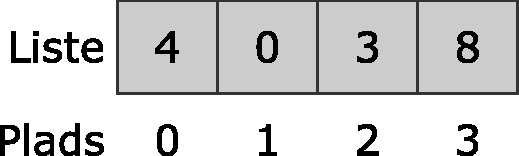
\includegraphics[width=0.6\textwidth]{figs/list.pdf}
	\end{center}

\end{frame}


\begin{frame}[fragile]{Indeksering i lister}
Vi kan indeksere med alle slags værdier:
\begin{columns}
	\column{0.4\textwidth}
	\begin{lstlisting}[style=python]
mylist = [4, 0, 3, 8]
x = 1
print(mylist[x])
print(mylist[len(mylist)-1])
	\end{lstlisting}
	\pause
	\column{0.4\textwidth}
	\begin{lstlisting}[style=python]
0
8
	\end{lstlisting}
\end{columns}

\end{frame}

\begin{frame}[fragile]{Slicing}
	Vi kan tage en del af en liste ved hjælp af slicing:
	\begin{columns}
		\column{0.4\textwidth}
		\begin{lstlisting}[style=python]
mylist= [4, 0, 3, 8]
print(mylist[1:3])
		\end{lstlisting}
		\pause
		\column{0.4\textwidth}
		\begin{lstlisting}[style=python]
[0, 3]
		\end{lstlisting}
	\end{columns}
	Bemærk her at element 1 og 2 printes. For \texttt{[n:m]} inkluderes det \texttt{n}'te element og det \texttt{m}'te ekskluderes.
\end{frame}


\begin{frame}[fragile]{Iteration af en liste}
	Et gennemløb af en liste er en typisk operation:
	\begin{columns}
		\column{0.4\textwidth}
		\begin{lstlisting}[style=python]
mylist= [4, 0, 3, 8]
for elm in mylist:
	print(elm)
		\end{lstlisting}
		\column{0.4\textwidth}
		\begin{lstlisting}[style=python]
4
0
3
8
		\end{lstlisting}
	\end{columns}
	Her er \texttt{elm} en variabel. Kan også gøres med de allerede lærte løkker som while- og forløkker.
\end{frame}

\begin{frame}[fragile]{Ændring af element}
	Lister er mutable. Dvs. vi kan ændre dets elementer.
	\begin{columns}
		\column{0.4\textwidth}
		\begin{lstlisting}[style=python]
mylist= [4, 0, 3, 8]
print(mylist)
mylist[0] = 7
print(mylist)
		\end{lstlisting}
		\column{0.4\textwidth}
		\begin{lstlisting}[style=python]
[4, 0, 3, 8]
[7, 0, 3, 8]
		\end{lstlisting}
	\end{columns}
	Bemærk igen at første plads i listen er plads nummer 0.
\end{frame}

\begin{frame}[fragile]{Listemetoder}
	Tilføj et element til en liste:
	\begin{columns}
		\column{0.4\textwidth}
		\begin{lstlisting}[style=python]
mylist= [4, 0, 3, 8]
print(mylist)
mylist.append(5)
print(mylist)
		\end{lstlisting}
		\column{0.4\textwidth}
		\begin{lstlisting}[style=python]
[4, 0, 3, 8]
[4, 0, 3, 8, 5]
		\end{lstlisting}
	\end{columns}
	\pause
	Fjern fra en liste
	\begin{columns}
		\column{0.4\textwidth}
		\begin{lstlisting}[style=python]
mylist = [4, 0, 3, 8]
print(mylist)
del(mylist[0])
print(mylist)
		\end{lstlisting}
		\column{0.4\textwidth}
		\begin{lstlisting}[style=python]
[4, 0, 3, 8]
[0, 3, 8]
		\end{lstlisting}
	\end{columns}
\end{frame}

\begin{frame}[fragile]{Listemetoder}
	Længde af en liste.
	\begin{columns}
		\column{0.4\textwidth}
		\begin{lstlisting}[style=python]
mylist = [4, 0, 3, 8]
x = len(mylist)
print(x)
		\end{lstlisting}
		\pause
		
		\column{0.4\textwidth}
		\begin{lstlisting}[style=python]
4
		\end{lstlisting}
	\end{columns}
	\pause
	Concatenation:
	\begin{columns}
		\column{0.4\textwidth}
		\begin{lstlisting}[style=python]
mylist1 = [1, 2]
mylist2 = [3, 4]
mylist3 = mylist1 + mylist2
print(mylist3)
		\end{lstlisting}
		\pause
		
		\column{0.4\textwidth}
		\begin{lstlisting}[style=python]
[1, 2, 3, 4]
		\end{lstlisting}
	\end{columns}
\end{frame}

\begin{frame}[fragile]{Listemetoder}
	Multiplication:
	\begin{columns}
		\column{0.4\textwidth}
		\begin{lstlisting}[style=python]
mylist1 = [1, 2]
mylist2 = mylist1 * 3
print(mylist2)
		\end{lstlisting}
		\column{0.4\textwidth}
		\begin{lstlisting}[style=python]
[1, 2, 1, 2, 1, 2]
		\end{lstlisting}
	\end{columns}
\pause
Hmm, minder det os om noget?...

	\pause
	Tjek om element i en liste:
	\begin{columns}
		\column{0.4\textwidth}
		\begin{lstlisting}[style=python]
mylist = [1, 2, 3, 4, 5]
print(2 in mylist)
print(7 in mylist)
		\end{lstlisting}
		\column{0.4\textwidth}
		\begin{lstlisting}[style=python]
True
False
		\end{lstlisting}
	\end{columns}
\end{frame}

\begin{frame}[fragile]{Lidt af det hele}
Et eksempel
	\begin{lstlisting}[style=python]
yndlings =  []
for i in range(3):
  x = int(input("Indtast et af dine yndlingstal\n"))
  yndlings.append(x)

if (7 in yndlings):
  print("7 er nice")
else:
  print("Du har ikke mit yndlingstal i din top 3 :(")
	\end{lstlisting}
\end{frame}


\begin{frame}[fragile]{Range}
Det kan være brugbart at tænke på \texttt{range} således:


\begin{lstlisting}[style=python]
range(5) == [0, 1, 2, 3, 4]
\end{lstlisting}

\pause
Når man kigger på 

\begin{columns}
	\column{0.4\textwidth}
	\begin{lstlisting}[style=python]
for i in range(5):
print(i)
	\end{lstlisting}
	\column{0.4\textwidth}
	\begin{lstlisting}[style=python]
0
1
2
3
4
	\end{lstlisting}
\end{columns}
\end{frame}


\begin{frame}[fragile]{Lidt af det hele}
Hvis man har brug for indekset af et element gør man ofte således:
\begin{lstlisting}[style=python]
mylist = [4, 0, 3, 8]
for i in range(len(mylist)):
  print("På plads " + str(i) + " er der " + str(mylist[i]))
\end{lstlisting}
\pause

Output:
\begin{lstlisting}[style=python]
På plads 0 er der 4
På plads 1 er der 0
På plads 2 er der 3
På plads 3 er der 8
\end{lstlisting}
\end{frame}


\begin{frame}{Want more?}
	Flere metoder og eksempler kan findes her:\\
	\url{https://docs.python.org/3/tutorial/datastructures.html}
\end{frame}

\end{document}
